\documentclass[12pt]{article}
\usepackage{graphics}
\usepackage[top=1in,bottom=1in,left=1in,right=1in]{geometry}
\usepackage{alltt}
\usepackage{array}	
\usepackage{graphicx}
\usepackage{tabularx}
\usepackage{verbatim}
\usepackage{setspace}
\usepackage{listings}

\usepackage{amssymb,amsmath, amsthm}
\usepackage{zed-csp}
\usepackage[cc]{titlepic}

\title{COMP 335: Introduction to Theoretical Computer Science\\
\ \\
Assignment 1}
\author{Nathan Grenier}
\date{\today \\ Fall 2024}

\begin{document}
\begin{spacing}{1.5}
	\maketitle

	\newpage

	\begin{enumerate}

		\item[1.] [15 Points] For each of the following statements write if the statement is TRUE or FALSE. If the statement is TRUE then provide a proof. If the statement is FALSE then provide a counter-example.

		      \begin{enumerate}

			      \item For every language $L$ we have $L^2 \subseteq L^3$

			            \noindent \textbf{Answer:} FALSE

			            \noindent \textbf{Counter Example:}

			            $\Sigma = \{a,b \}$

			            $L=\{a, ab \}$

			            $L^2=LL=\{aa, aab, aba, abab \}$

			            $L^3=L^2L=\{aaa, aaaba, aaba, aabab, abaa, abaab, ababa, ababab \}$

			            $\{aa, aab, aba, abab \} \not\subseteq \{aaa, aaaba, aaba, aabab, abaa, abaab, ababa, ababab \}$

			            $\therefore L^2 \not\subseteq L^3$


			      \item For every two languages $L_1$ and $L_2$ we have $(L_1 \cup L_2)^* \subseteq (L_1L_2)^*$

			            \noindent \textbf{Answer:} FALSE

			            \noindent \textbf{Counter Example:}

			            $L_1 = \{x \}$, $L_2= \{y \}$, $\Sigma = \{x,y \}$

			            $L_1 \cup L_2 = \{x,y \}$, $L_1L_2 = \{xy \}$

			            $(L_1 \cup L_2)^* = \{\lambda \} \cup \{x,y \} \cup \{xx, xy, yx, yy \} \cup \dots$

			            $(L_1L_2)^* = \{\lambda \} \cup \{xy \} \cup \{xyxy \} \cup \{xyxyxy \} \cup \dots$

			            $\therefore (L_1 \cup L_2)^* \not\subseteq (L_1L_2)^*$

			            \newpage

			      \item Let $L_1$ and $L_2$ be two languages such that $\lambda \in L_1 \cap L_2$. Then it holds that $(L_1L_2)^* = (L_2L_1)^*$

			            \noindent \textbf{Answer:} TRUE

			            \noindent \textbf{Direct Proof:}

			            \begin{enumerate}
				            \item[1.] $\subseteq$:

				                  $\rightarrow$ Let $w \in (L_1L_2)^*$

				                  $\rightarrow$ $w$ is of the form: $w = x_1y_1x_2y_2 \dots x_ny_n$ where $x_i \in L1 \land y_i \in L_2$

				                  $\rightarrow$ Since $\lambda \in L_1 \sup L_2$ then $w = x_1 \lambda y_1 \lambda x_2 \lambda y_2 \dots x_n \lambda y_n$

				                  $\rightarrow$ Format the string $w = (\lambda x_1)y_1(\lambda x_2)y_2 \dots (\lambda x_n)y_n$

				                  $\rightarrow$ Using the associative property of string
				                  concatenation

				                  ($(a\times b) \times c = a \times (b \times c)$), we can rewrite the string as $w = (y_1x_1)\lambda(y_2x_2)\lambda \dots (y_nx_n)\lambda$

				                  $\rightarrow$ $w = (y_1'x_1')(y_2'x_2') \dots (y_n'x_n')$ where $x_i' \in L_1 \land y_i' \in L_2$

				                  $\therefore$ $w \in (L_2L_1)^*$

				            \item[2.] $\supseteq$:

				                  $\rightarrow$ Let $w \in (L_2L_1)^*$

				                  $\rightarrow$ $w$ is of the form: $w = y_1x_1y_2x_2 \dots y_nx_n$ where $x_i \in L1 \land y_i \in L_2$

				                  $\rightarrow$ Since $\lambda \in L_1 \sup L_2$ then $w = y_1 \lambda x_1 \lambda y_2 \lambda x_2 \dots y_n \lambda x_n$

				                  $\rightarrow$ Format the string $w = (\lambda y_1)x_1(\lambda y_2)x_2 \dots (\lambda y_n)x_n$

				                  $\rightarrow$ Using the associative property of string
				                  concatenation

				                  ($(a\times b) \times c = a \times (b \times c)$), we can rewrite the string as $w = (x_1y_1)\lambda(x_2y_2)\lambda \dots (x_ny_n)\lambda$

				                  $\rightarrow$ $w = (x_1'y_1')(x_2'y_2') \dots (x_n'y_n')$ where $x_i' \in L_1 \land y_i' \in L_2$

				                  $\therefore$ $w \in (L_1L_2)^*$

			            \end{enumerate}

		      \end{enumerate}

		      \newpage

		\item[2.] [10 Points] The following is a transition diagram for a DFA over the alphabet $\Sigma = \{0,1\}$. Answer the following questions about this automaton:

		      \begin{figure}[h!]
			      \centering
			      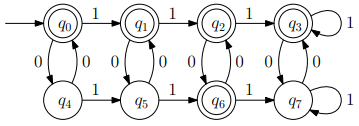
\includegraphics[width=0.6\textwidth]{img/q2/q2_automata.png}
		      \end{figure}

		      \begin{enumerate}
			      \item What is the start state? What is the set of accept states?

			            \noindent \textbf{Answer:}

			            Start State = $q_0$

			            Accept States = $\{q_0, q_1, q_2, q_3, q_6\}$

			      \item What is the sequence of states the DFA goes through on input 101100?

			            \noindent \textbf{Answer:} $(q_0, q_1, q_5, q_6, q_7, q_3, q_7)$

			      \item Does the machine accept every string $w$ that contains exactly two 1s? Why or why not?

			            \noindent \textbf{Answer:} $L = \{0^*10^*10^* \}$

			            Yes. Since the string always contains exactly two 1s, the machine traverses to one of these states $\{q_2, q_6 \}$. Since $q_2, q_6 \in F$ and only 0 appear in the string after consuming both 1s, the machine can only transition between these acceptance states.

			      \item Does the machine reject every string $w$ that has odd number of 0s? Why or why not?

			            \noindent \textbf{Answer:} $L = \{w \in \Sigma^* : \text{Where $n_0(w)$ mod $2 \neq 0$} \}$

			            No. Since there's an odd number of 0s, the any string will always terminate in the following states $\{q_4, q_5, q_6, q_7 \}$. However, not all of these states are acceptance states (only $q_6 \in F$). Therefore, depending on how many 1s are present in the string, we may or may not reach an acceptance state.

			            \textbf{Counter Example:} $w = 011$, Final State = $q_6$

			      \item Describe the language accepted by the machine using the set builder notation.

			            \noindent \textbf{Answer:}
			            \begin{equation}
				            \begin{split}
					            L = & \{w \in \Sigma^* : \text{Where } n_0(w) \mod 2 = 0 \} \lor \\ & \{w \in \Sigma^+ : \text{Where } n_0(w) \mod 2 \neq 0 \land n_1(w) = 2 \}
				            \end{split}
			            \end{equation}

		      \end{enumerate}

		      \newpage

		\item[3.] [30 Points] For each of the following languages, give a DFA that accepts it.

		      \begin{enumerate}
			      \item $\{ba^nb^m : n \geq 3, m \geq 2 \}$

			            \noindent \textbf{Answer:}

			            \begin{figure}[h!]
				            \centering
				            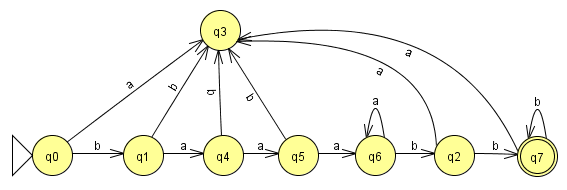
\includegraphics[width=0.75\textwidth]{img/q3/q3_a.png}
			            \end{figure}

			      \item $\{w \in \{a,b \}^* : \text{every maximal substring } w \text{ consisting entirely of symbols } a \\ \text{ is of length exactly 3} \}$

			            \noindent \textbf{Answer:}

			            \begin{figure}[h!]
				            \centering
				            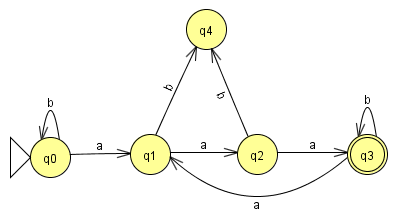
\includegraphics[width=0.6\textwidth]{img/q3/q3_b.png}
			            \end{figure}

			            \newpage

			      \item $\{w \in \{a,b \}^* : \text{$w$ does not contain $bab$ as a substring} \}$

			            \noindent \textbf{Answer:}

			            \begin{figure}[h!]
				            \centering
				            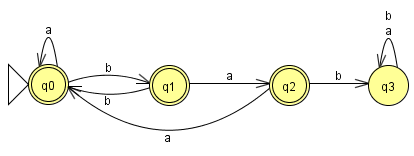
\includegraphics[width=0.6\textwidth]{img/q3/q3_c.png}
			            \end{figure}

			      \item $\{w \in \{a,b \}^* : \text{$w$ begins with bb and $n_b(w)$ mod 3 = 0} \}$

			            \noindent \textbf{Answer:}

			            \begin{figure}[h!]
				            \centering
				            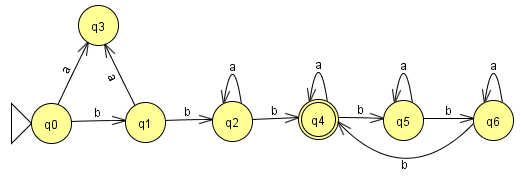
\includegraphics[width=0.75	\textwidth]{img/q3/q3_d.png}
			            \end{figure}

			            \newpage

			      \item $\{a^mb^n : mn > 4\}$

			            \noindent \textbf{Answer:}

			            \begin{figure}[h!]
				            \centering
				            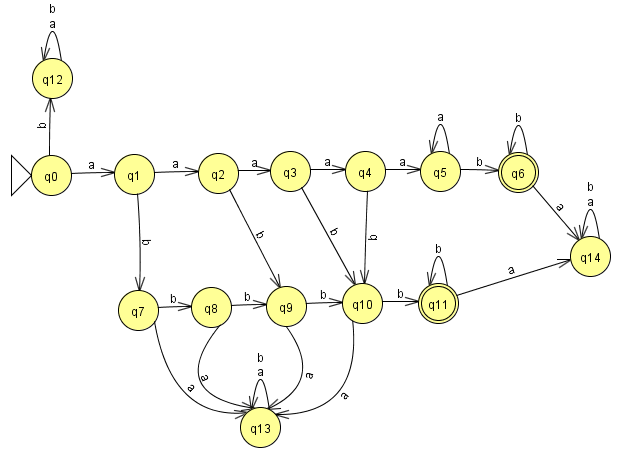
\includegraphics[width=0.75\textwidth]{img/q3/q3_e.png}
			            \end{figure}

			      \item $\{vwv^R : v,w \in \{a,b \}^* \text{ and} |v| = 2 \}$

			            \noindent \textbf{Answer:}

			            \begin{figure}[h!]
				            \centering
				            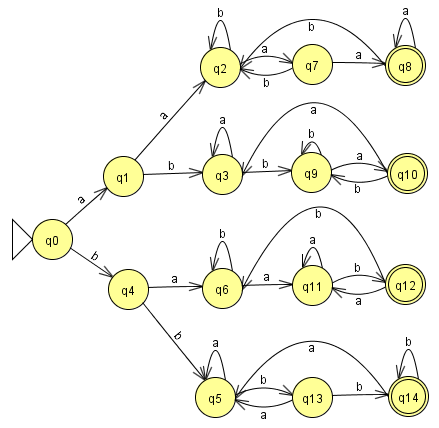
\includegraphics[width=0.55\textwidth]{img/q3/q3_f.png}
			            \end{figure}
		      \end{enumerate}

	\end{enumerate}

\end{spacing}

\end{document}